%
% CMPT 300: Operating Systems I - A Course Overview
%
% Author: Jeffrey Leung
%

\documentclass[10pt, oneside, letterpaper, titlepage]{article}

\usepackage{amsmath}
\usepackage{caption}
\usepackage[ampersand]{easylist}
	\ListProperties(
		Progressive*=5ex,
		Space=5pt,
		Space*=5pt,
		Style1*=\textbullet\ \ ,
		Style2*=\begin{normalfont}\begin{bfseries}\textendash\end{bfseries}\end{normalfont} \ \ ,
		Style3*=\textasteriskcentered\ \ ,
		Style4*=\begin{normalfont}\begin{bfseries}\textperiodcentered\end{bfseries}\end{normalfont}\ \ ,
		Style5*=\textbullet\ \ ,
		Style6*=\begin{normalfont}\begin{bfseries}\textendash\end{bfseries}\end{normalfont}\ \ ,
		Style7*=\textasteriskcentered\ \ ,
		Style8*=\begin{normalfont}\begin{bfseries}\textperiodcentered\end{bfseries}\end{normalfont}\ \ ,
		Hide1=1,
		Hide2=2,
		Hide3=3,
		Hide4=4,
		Hide5=5,
		Hide6=6,
		Hide7=7,
		Hide8=8 )
\usepackage{geometry}
	\geometry{margin=1.2in}
\usepackage{graphicx}
	\graphicspath{ {img/} }
\usepackage[colorlinks=true, linkcolor=blue]{hyperref}
\usepackage{listings}
\usepackage{lmodern} % Allows the use of symbols in font size 10; http://ctan.org/pkg/lm
\usepackage{textcomp} % Allows the use of \textbullet with the font
\usepackage{tikz}
\usepackage{verbatim}

\renewcommand{\arraystretch}{1.5}
\renewcommand{\familydefault}{\sfdefault}

\title{CMPT 300: Operating Systems I \\\medskip \Large A Course Overview}
\author{Jeffrey Leung \\ Simon Fraser University}
\date{Fall 2018}

\begin{document}

	\maketitle
	\tableofcontents
	\clearpage

	%
% CMPT 213: Object Oriented Design in Java - A Course Overview
% Section: Introduction
%
% Author: Jeffrey Leung
%

\section{Introduction}
	\label{sec:introduction}
\begin{easylist}

& Standards:
	&& Make fields private when possible

& Commenting:
	&& Comment purpose of a class
	&& Name fields/methods/parameters so comments are unnecessary

& When possible, convert strings to non-string types internally for consistency

& \textbf{Clean code:} Code which is correct, easy to read/maintain, and conforms to a standard

& Software design:
	&& 4 steps:
		&&& Requirements
		&&& Design and implementation
		&&& Verification
		&&& Evolution
	&& Designing involves identifying classes, responsibilities, and relationships to create a diagram
	&& Implementation process options:
		&&& \textbf{Skeleton code:} Beginning minimal parts/features of a system
		&&& \textbf{Component-wise:} Creating components one at a time
	&& Methods of integrating code from multiple people:
		&&& \textbf{Continual integration:} Gradual system growth by constantly integrating changes
		&&& \textbf{Big Bang integration:} Building all parts separately without integrating until the end

& \textbf{Feature envy:} Characteristic of a class which relies heavily on another class
& Warning sign: Characteristic of a method which operates more strongly on another object than its own
& \textbf{Deprecation:} State where a public interface is no longer supported or recommended, and is slated to be removed in the future


& \textbf{try-catch:} Structure which watches for an exception and handles it
	&& Only one exception can be live at a given time
	&& \textbf{finally clause:} Optional clause after catch clauses which is executed regardless of the result
		&&& If exception is thrown, the finally clause is executed immediately afterwards
	&& \textbf{try-with-resources:} Block which cleans up a resource when a try block exits

& Exception: Issue which may be fixable and is not out of the software's control
	&& \textbf{Checked exception:} Exception which must be caught or listed in a throws clause
	&& \textbf{Unchecked exception:} Exception which will automatically propagate and does not require catching
		&&& E.g. RuntimeException
		&&& Preferred as it does not require modification of methods between try/catch, which decouples code

\end{easylist}
\clearpage

	%
% CMPT 300: Operating Systems I - A Course Overview
% Section: Processes
%
% Author: Jeffrey Leung
%

\section{Processes}
	\label{sec:processes}
\begin{easylist}

& \textbf{Process:} Program which is loaded in memory and currently being executed (i.e. the required OS structures exist)
	&& Consists of a program counter, stack (which includes local variables and return address), and data location/area (which includes global variables and dynamically allocated memory) (see figure~\ref{fig:processes:process-data})
	\begin{figure}[!htb]
		\centering
		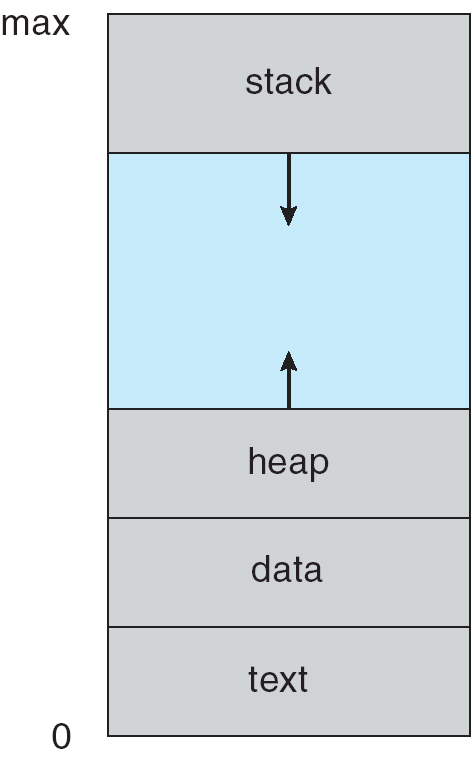
\includegraphics[width=0.3\textwidth]{process-data}
		\caption{Process Data}
		\label{fig:processes:process-data}
	\end{figure}
	&& Created by a parent process; may create children processes

& \textbf{Process state:} Current execution stage of a process
	&& New, running, waiting (for an event), ready (waiting for CPU), terminated
& \textbf{Process Control Block (PCB):} Set of data about a particular process
	&& Used to switch the CPU between processes
	&& Data includes process state, program counter, CPU registers, CPU scheduling information, memory management information, I/O status information

& Managed in scheduling queues
	&& \textbf{Ready queue:} Set of processes in memory which are ready to execute
	&&& \textbf{Device queue:} Set of processes in memory which are waiting for an I/O device
	&& See figure~\ref{fig:processes:scheduling-queues}
	\begin{figure}[!htb]
		\centering
		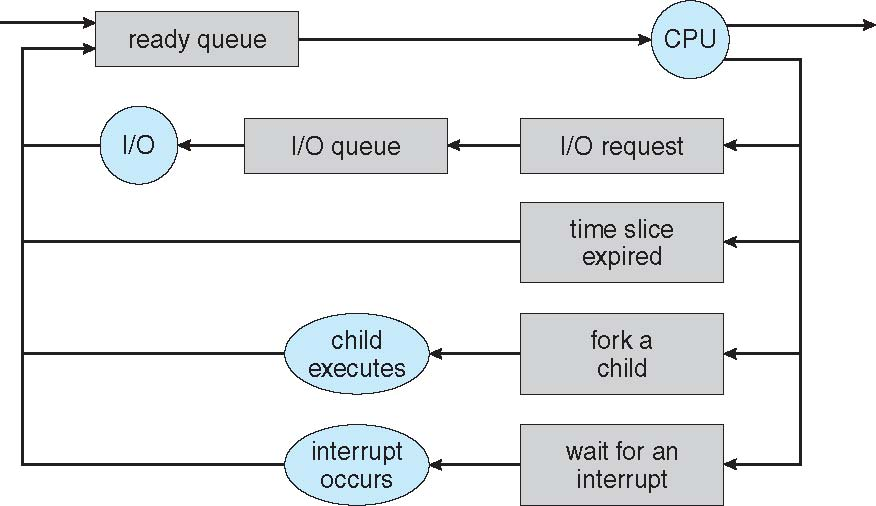
\includegraphics[width=0.7\textwidth]{scheduling-queues}
		\caption{Scheduling Queues}
		\label{fig:processes:scheduling-queues}
	\end{figure}

& \textbf{Context switch:} CPU changing from one process to another
	&& State of the first process is saved in a PCB in memory; state of the second process from another PCB in memory is loaded into the registers
	&& \textbf{CPU state:} Values of the CPU registers
		&&& Includes program counter and stack counter
	&& Overhead with no work done
	&& Usually several milliseconds
	&& Some systems use multiple register sets which can be easily switched between using pointers

&& \textbf{Fork:} System call executed by a process (parent) which creates a new process (child)
	&&& Child is a copy of the parent
	&&& Child loads another program using the \lstinline[columns=fixed]{exec()} system call % [ Left bracket to fix syntax highlighting error by Texmaker
	&&& Parent waits for children to exit, or aborts the execution of its children
		&&&& \textbf{Cascade termination:} Abortion of the children of a child process
		&&&& OS deallocates resources
		&&&& Data is returned to parent via \lstinline[columns=fixed]{wait()} % [ Left bracket to fix syntax highlighting error by Texmaker
		&&&& \textbf{Zombie process:} Process which has been terminated but whose parent has not yet called \lstinline[columns=fixed]{wait()} % [ Left bracket to fix syntax highlighting error by Texmaker
			&&&&& Return value held temporarily in memory
		&&&& \textbf{Orphan process:} Process which is running but its parent has exited (without calling \lstinline[columns=fixed]{wait()}) % [ Left bracket to fix syntax highlighting error by Texmaker
			&&&&& \textbf{Adoption:} Changing the parent of an orphaned process to the \lstinline[columns=fixed]{init} process % [ Left bracket to fix syntax highlighting error by Texmaker

\end{easylist}
\subsection{Threads}
	\label{subsec:processes:threads}
\begin{easylist}

& \textbf{Thread:} Sequence of instructions which the CPU can execute as a unit
	&& Tracked by program counter, register set, and stack
	&& Created by system call \lstinline[columns=fixed]{clone()} % [ Left bracket to fix syntax highlighting error by Texmaker
		&&& Can be parameterized to share or duplicate resources
	&& Equivalent to processes in Linux

& \textbf{Multithreading:} Utilization of multiple threads by a single process
	&& Threads of the same process share a code section, data section, and OS resources
	&& Benefits: Responsive, shares resources, scalable
	&& If \lstinline[columns=fixed]{fork()} is called by a process with multiple threads, all threads are duplicated unless \lstinline[columns=fixed]{exec()} is called immediately afterwards

& \textbf{User-level thread:} Thread operating only in user space
	&& Data structures and thread operations are in user level/mode only
	&& Kernel is not aware of user-level threads
& \textbf{Kernel-level thread:} Thread operating only in kernel space
	&& Data strcutures and thread operations are in kernel level/mode (requiring system calls)
	&& Provided by the kernel

& Mappings from user threads to kernel threads:
	&& One-to-one: User level threads are mapped individually to kernel threads
		&&& Pros: Increased concurrency (multiprocessors can be used); one thread cannot block another
		&&& Con: Significant overhead for thread resource usage and management
	&& Many-to-one: Threads are managed in user level to have several user threads map to a single kernel thread
		&&& Pro: Faster thread management due to no switching or system calls
		&&& Cons: A single thread can block all other threads; incompatible with multiprocessors
		&&& E.g. Solaris Green Threads library
	&& Many-to-many: Multiple user threads are mapped to multiple kernel threads
		&&& \textbf{Thread scheduler:} User-level module which manages mapping of user threads to kernel threads
			&&&& \textbf{Upcall:} Notification by kernel when a user thread blocks so another user thread can use the free kernel thread
				&&&&& Complex processing to redirect other threads, nearly duplicating kernel-level work
			&&&& Pros: Increased concurrency and flexibility
			&&&& Con: Difficult to implement

& E.g. POSIX Pthreads API specification used in UNIX systems
	&& \lstinline[columns=fixed]{pthread_create()} blocks until \lstinline[columns=fixed]{pthread_exit()}
	&& \lstinline[columns=fixed]{pthread_join()} combines the two threads % [ Left bracket to fix syntax highlighting error by Texmaker

& \textbf{Thread pool:} Limited set of user-level threads which are either available for use or in use
	&& Removes the overhead of creating new threads
	&& When a new request is created, an inactive thread is pulled from the pool to service the task
	&& Used commonly in web servers to service incoming requests

\end{easylist}
\subsection{Signals}
	\label{subsec:processes:signals}
\begin{easylist}

& \textbf{Signal:} Event notification sent to a process
	&& \textbf{Synchronous signal:} Signal to the same process which caused the signal
		&&& Specific to the thread which caused the signal
		&&& E.g. Illegal memory access
	&& \textbf{Asynchronous signal:} Signal from one process to another
		&&& Delivered to all threads of the process
		&&& E.g. Cancelling a running process with \lstinline[columns=fixed]{Ctrl-C} % [ Left bracket to fix syntax highlighting error by Texmaker

& \textbf{Signal handler:} OS or user-defined module which processes a signal

& Comparison to \hyperref[sec:introduction]{interrupts} (see figure~\ref{fig:processes:comparison}):

\end{easylist}
\begin{figure}[!htb]
	\centering
	\caption{Comparison between Interrupts and Signals}
	\label{fig:processes:comparison}
	\begin{tabular}{ r | p{6cm} p{6cm} }
		& Interrupts & Signals \\
		\hline
		Initiated by &
		\parbox[t]{5cm}{CPU (e.g. division by 0),\\I/O devices (e.g. user input), or\\software (e.g.system call)} &
		\parbox[t]{5cm}{Kernel (e.g. SIGIO) or\\process (e.g. SIGKILL)} \\
		Handled by &
		Interrupt Service Routine in kernel space &
		\parbox[t]{5cm}{Kernel (default) or\\process (manual override)\\in user space} \\
		Continuation &
		May map to signals and deliver to processes for specific handling &
		May have complex logic to call other functions in kernel
	\end{tabular}
\end{figure}
\begin{easylist}

\end{easylist}
\clearpage
	%
% CMPT 300: Operating Systems I - A Course Overview
% Section: Scheduling
%
% Author: Jeffrey Leung
%

\section{Scheduling}
	\label{sec:scheduling}
\begin{easylist}

& Process execution switches between bursts of CPU execution and I/O wait
	&& \textbf{I/O bound process:} Process which spends more time in I/O waits than CPU execution
	&& \textbf{CPU bound process:} Process which spends more time in CPU execution than I/O waits

& %TODO diagram

& \textbf{Long-term/job scheduler:} Component which decides which processes should be moved to the ready queue, to maintain a balanced mix of I/O-bound and CPU-bound processes
	&& Controls degree of concurrency/multiprogramming
	&& Slow; invoked infrequently
& \textbf{Midterm scheduler:} Component which holds partially-executed processes which are not in the ready queue %TODO

& \textbf{Short-term/CPU scheduler:} Component which decides which processes from the ready queue the CPU should perform work for
	&& Quick; invoked frequently (every several milliseconds)
	&& \textbf{Nonpreemptive:} Process which can only stop during CPU execution by terminating or by waiting (e.g. I/O request, child termination)
	&& \textbf{Preemptive:} Process which can be forcefully stopped (preempted) during CPU execution by the OS (e.g. to run a higher-level process)
		&&& More difficult to implement
			&&&& Needs to maintain consistency of data shared between processes and kernel data structures (e.g. I/O queues)
			&&&& Needs hardware support (e.g. timers)

& \textbf{Dispatcher:} Component which allocates the CPU to various processes by switching context, switching user mode, jumping to the specified location in the process, and restarting execution
	&& \textbf{Dispatch latency:} Time required for the dispatcher to switch tasks

\end{easylist}
\subsection{Scheduling Algorithms}
	\label{subsec:scheduling:algorithms}
\begin{easylist}


& Criteria:
	&& Maximize CPU utilization
	&& Maximize throughput
	&& Minimize first response time
	&& Minimize waiting time (time before a process starts exeuction)
	&& Minimize job turnaround time

& \textbf{Convoy effect:} Suboptimal situation where a long process blocks the CPU, requiring shorter processes to wait
	&& Utilization of CPU and device is low

& \textbf{First-Come, First-Served (FCFS):} CPU scheduling algorithm which prioritizes processes based on when they are placed in the queue
	&& Tasks which take longer will block other tasks; a CPU-bound process would block I/O-bound processes
	&& Examples:
		&&& For tasks P\textsubscript{1} = 24ms, P\textsubscript{2} = 3ms, P\textsubscript{3} = 3ms in the given order (see diagram~\ref{fig:scheduling:gantt-1}), the average waiting time is $\frac{0 + 24 + 27}{3} = 17 \text{ms}$
		
\begin{figure}[!htb]
	\centering
	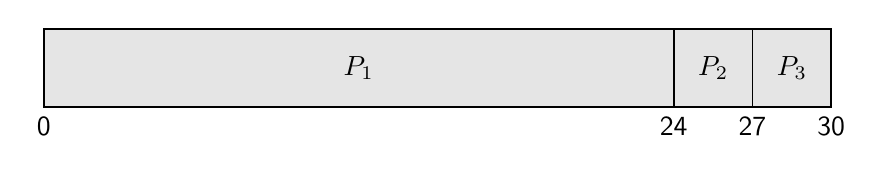
\begin{tikzpicture}[line width=.7pt]
		\draw[fill=gray!20] (0,0)node[below]{0} rectangle(8,1);
		\draw[fill=gray!20] (8,0)node[below]{24} rectangle(9,1);
		\draw[fill=gray!20] (9,0)node[below]{27} rectangle (10,1) node[below,yshift=-1cm]{30};
		\path (4,0.5) node{$P_1$} (8.5,0.5) node{$P_2$} (9.5,0.5) node{$P_3$};
	\end{tikzpicture}
	\caption{FCFS Gantt Chart for P\textsubscript{1} = 24ms, P\textsubscript{2} = 3ms, P\textsubscript{3} = 3ms}
	\label{fig:scheduling:gantt-1}
\end{figure}

		&&& For tasks P\textsubscript{2} = 3ms, P\textsubscript{3} = 3ms, P\textsubscript{1} = 24ms in the given order, the average waiting time is $\frac{0 + 3 + 6}{3} = 3 \text{ms}$


& \textbf{Shortest Job First (SJF):} CPU scheduling algorithm which prioritizes processes based on shortest execution time (without preempting currently running processes)
	&& Provably optimal in giving minimum average waiting time for a given set of processes
	&& Length of next CPU burst is available for long-term scheduling but not available for short-term scheduling
	&& Time of execution is approximated through prediction from previous executions %TODO
	&& Examples:
		&&& For tasks: %TODO
	&&& Time prediction %TODO
& \textbf{Shortest Remaining Time First (SRTF):} CPU scheduling algorithm which prioritizes processes based on the least execution time remaining, switching between processes when necessary
	&& Examples: %TODO
& \textbf{Round Robin:} CPU scheduling algorithm which provides a unit of time (\textit{q)}) for each process before moving to the next process
	&& \textbf{Time quantum} ($q$): Unit of CPU time (10-100 ms) for which a process can execute
		&&& For $n$ processes in the ready queue, each process receives $\frac{1}{n}$ of CPU time
		&&& $q$ and context switch time %TODO
	&& Process is moved to end of (circular) ready queue once its time is finished
	&& Better response time and higher average turnaround time (vs. SJF)

& \textbf{Priority scheduling:} CPU process scheduling which allocates work depending on a priority level
	&& SJF is when the priority is the inverse of the CPU burst length
	&& \textbf{Starvation:} Failure to allocate a low-priority process
		&& \textbf{Aging:} %TODO

& \textbf{Multilevel queue scheduling:} Scheduling design with multiple prioritized ready queues, each with its own scheduling algorithm
	&& %TODO

& \textbf{Multiprocessor scheduling:}
	&& Divide load among multiple processors
	&& \textbf{Asymmetric multiprocessor:} Multiprocessor scheduling strategy where one master processor handles all scheduling
	&& \textbf{Symmetric multiprocessor:} Multiprocessor scheduling strategy where %TODO
		&&& Issues:
			&&&& \textbf{Processor affinity:} Binding and unbinding of a process to the CPU
				&&&&& When a process is migrated to a new processor, the old cache must be invalidated and the new cache must be re-populated which has a performance penalty
			&&&& \textbf{Load balancing:} Workload distribution among various processors
				&&&&& \textbf{Push migration:} Task repeatedly checks all processors and moves tasks to evenly distribute them
				&&&&& \textbf{Pull migration:} Idle processor taking a task from a busy processor
			&&&& Tradeoff between processor affinity and load balancing

& \textbf{Real-time scheduling:} %TODO

& \textbf{Completely Fair Scheduler:} %TODO
	&& \textbf{Target latency:} Duration of time during which every runnable task should be executed at least once
		&&& \textbf{Nice value:} Duration of time during which... %TODO

& How algorithms are designed:
	&& Use deterministic modelling to run algorithms on workloads
	&& Use queuing models and theory to analyze algorithms (using typically unrealistic assumptions)
	&& Use a simulator to model systems (using a synthetic workload or traces from real systems)
		&&& Expensive and time-consuming

\end{easylist}
\clearpage
	%
% CMPT 300: Operating Systems I - A Course Overview
% Section: Inter-Process Communication
%
% Author: Jeffrey Leung
%

\section{Inter-Process Communication}
	\label{sec:interprocess}
\begin{easylist}

& \textbf{Inter-process communication (IPC):} Sharing of information from one process to another
	&& Purposes:
		&&& Faster computation
		&&& Increased modularity
		&&& Increased convenience

& \textbf{Shared memory:} Method of IPC in which a single memory space is used by multiple processes
	&& Processes attach the shared memory space created by another process to their own address space
	&& Pros: Fast, convenient
	&& Cons: Requires synchronization to prevent conflicts
	&& Implementations (POSIX): \lstinline[columns=fixed]{shm_open()} to create a shared memory space and \lstinline[columns=fixed]{mmap()} to create a mapping from a process to the shared space

& \textbf{Message passing:} Method of IPC in which a process sends a message to another process through the kernel
	&& Can be to a process directly or can use constructs such as ports, mailboxes
	&& Process can block until a response is received
	&& Unsent messages may buffer and be placed in a waiting queue
	&& Diagram: See figure~\ref{fig:ipc-message-passing}
	&& Pros: No conflicts possible
	&& Cons: Slow, requires overhead through system calls and kernel
	
	\begin{figure}[!htb]
		\centering
		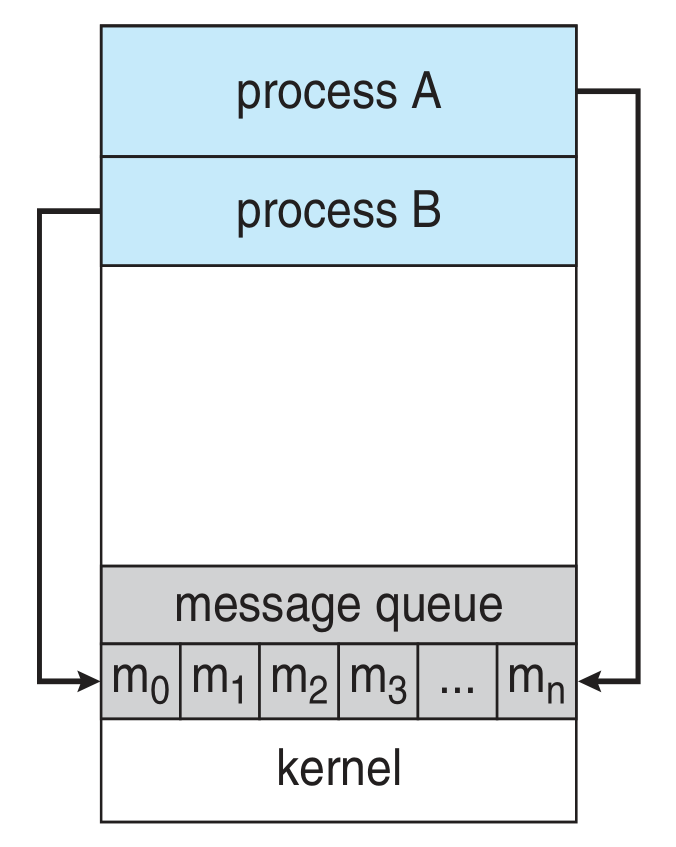
\includegraphics[width=0.2\textwidth]{ipc-message-passing}
		\caption{Diagram of message passing}
		\label{fig:ipc-message-passing}
	\end{figure}

\end{easylist}
\clearpage
	%
% CMPT 433: Embedded Systems - A Course Overview
% Section: Synchronization
%
% Author: Jeffrey Leung
%

\section{Synchronization}
	\label{sec:synchronization}
\begin{easylist}

& \textbf{Process:} Program which has a dedicated address space
	&& \textbf{Virtual access space:} Component of a process which is an abstracted memory location
	&& \textbf{fork():} Command which duplicates the address space of the current process
	&& \textbf{exec():} Set of commands which replaces the current process with an executable file

& \textbf{Thread:} Program which shares an address space with other instances of the same program
	&& Threads of the same process share a virtual access space, including global variables
& \textbf{Mutex:} Data structure which prevents simultaneous access to volatile data which may be changed
	&& \textbf{Critical section:} Section of code which can only be running once at a time
		&&& Keep critical sections as minimal as possible
& \textbf{Pipe:} Unidirectional data stream for inter-thread/process communication

\end{easylist}
\clearpage


	%
% CMPT 300: Operating Systems I - A Course Overview
% Section: 
%
% Author: Jeffrey Leung
%

\section{Deadlocks}
	\label{sec:deadlocks}
\begin{easylist}

& \textbf{Resource:} Limited-quantity component which is needed by a process (e.g. CPU time, memory space, I/O device access)
	&& Processes request (and block if resource is not free), use, and release a resource

& \textbf{Deadlock:} Situation where a set of blocked processes hold a resource and each needs to acquire a resource held by another process in the set
	&& Fundamental conditions:
		&&& \textbf{Mutual exclusion:} Natural condition where a single resource can be held by no more than one process
		&&& \textbf{Hold and wait:} Condition where a process holds a resource and waits to acquire another
		&&& \textbf{No preemption:} Condition where a process cannot be preempted during execution to release its resources
		&&& \textbf{Circular wait:} Condition where there exists a set of processes ${P_0, P_1, \ldots, P_n}$ such that $P_m$ is waiting for a resource held by $P_{m+1}$ where $m \neq n$, and $P_n$ is waiting for a resource held by $P_0$

& Resource Allocation Graph (RAG) %TODO

& Safety condition: There exists a sequence of all processes ${P_1, P_2, \ldots, P_n}$ such that each $P_i, 1 \leq i \leq n$, the resources that $P_i$ will request can be satisfied by the currently available resources in addition to the resources held by all $P_j, 1 \leq j < i$.

& \textbf{Deadlock prevention:} Strategies to prevent deadlocks through disallowing a specific process behaviour to disable one of the deadlock conditions
	&& Preventing hold and wait: A process may only hold one resource at a time (results in low resource utilization)
	&& Preventing hold and wait: A process is allocated all its resources before execution (results in starvation)
	&& Allowing preemption: A process may be preempted to lose its resources if the next resource request will not be satisfied, or if another process requires its resources (results in failure to maintain atomicity of operations due to resources which cannot easily save states)
	&& Preventing circular wait: All resource types have a total ordering and enforce process requests in a relative order
	
& \textbf{Deadlock avoidance:} Strategy to prevent deadlocks through forcing a process to wait if its resource allocation will create a deadlock

& \textbf{Deadlock detection and recovery:} Strategy to detect the occurrence of a deadlock in the system and eliminate processes until the deadlock is removed

\end{easylist}
\clearpage
	%
% CMPT 300: Operating Systems I - A Course Overview
% Section: Memory Management
%
% Author: Jeffrey Leung
%

\section{Memory Management}
	\label{sec:memory-management}
\begin{easylist}

& Code location can be absolute if memory location is known during compile time, or relocatable otherwise

& \textbf{Physical address:} Location in physical memory accessed by the memory unit
& \textbf{Logical/virtual address:} CPU-managed location in memory 
	&& Different from physical address if addresses are bound during execution
	&& \textbf{Memory Management Unit (MMU):} Hardware component which maps virtual addresses to physical addresses during runtime
		&&& Ensures separation and protection of memory areas
		&&& Basic components: Base and limit register

\end{easylist}
\subsection{Contiguous Allocation}
	\label{subsec:memory-management:contiguous-allocation}
\begin{easylist}

& Allocation algorithms:
	&& \textbf{First-fit algorithm:} Allocating memory in the first available sufficiently-sized hole
	&& \textbf{Best-fit algorithm:} Allocating memory in the smallest sufficiently-sized hole to create the smallest possible remaining hole
		&&& Requires searching the entire memory space
	&& \textbf{Worst-fit algorithm:} Allocating memory in the largest sufficiently-sized hole to create the largest possible remaining hole
		&&& Requires searching the entire memory space

& \textbf{External fragmentation:} Situation where the memory space exists to fulfill a request but it is not contiguous
	&& \textbf{Memory compaction:} Method to solve external fragmentation which places all free memory together
		&&& Only possible if addresses are bound during execution

\end{easylist}
\subsection{Paging}
	\label{subsec:memory-management:paging}
\begin{easylist}

& \textbf{Page:} Fixed-size, contiguous logical memory unit for non-contiguous memory allocation
	&& \textbf{Frame:} Fixed-size, contiguous physical memory unit for non-contiguous memory allocation
		&&& Associated 1:1 with each page

& Components of addresses:
	&& \textbf{Page number:} Component which contains the base address of a page in physical memory
	&& \textbf{Page offset:} Component which contains an offset of the base address sent to the MMU
	&& For $m, n$ where the address space is $2^m$ and the page size has $2^n$ entries, the number of pages is $\frac{2^m}{2^n} = 2^{m-n}$, the address has $m$ bits, the page number has $m-n$ bits, and the page offset has $n$ bits
	&& Size: Power of 2 (so that the page number and offset can be easily navigated)

& \textbf{Page table:} Set of translations from logical memory to physical memory
	&& Allows partitioning of physical memory and linkage with virtual memory in arbitrary ordering
	&& Specific to each process
	&& Located through the page table base register
	&& Requires two memory accesses (one for page table, one for instruction)
	&& Includes protection bits to specify if a page is read-only/read-write/execute-only, or if a page is valid/invalid access for the process
	&& Diagram: See figure~\ref{fig:paging:page-table-1}

	\begin{figure}[!htb]
		\centering
		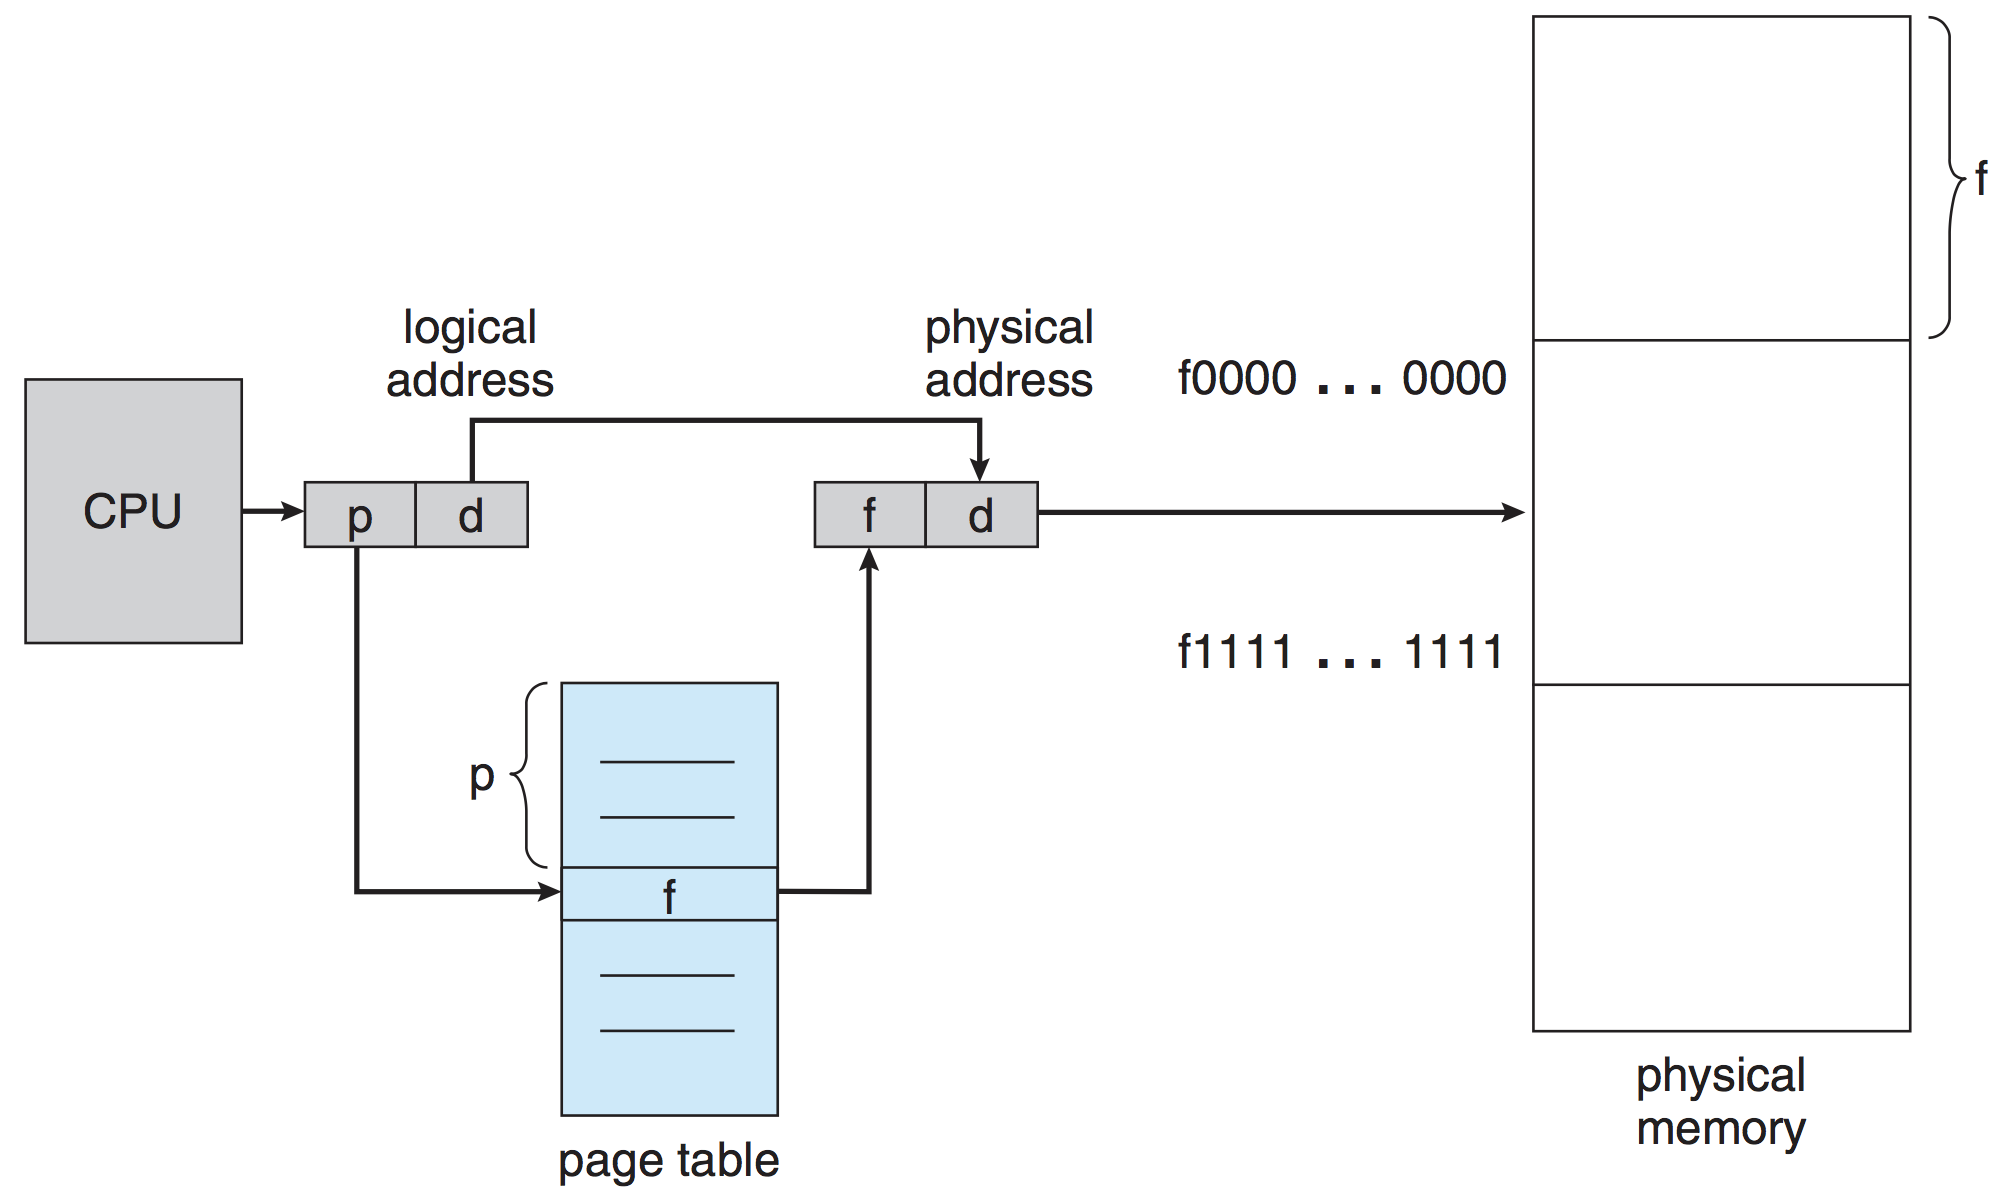
\includegraphics[width=0.7\textwidth]{page-table-1}
		\caption{Diagram of a Page Table}
		\label{fig:paging:page-table-1}
	\end{figure}
	
	&& Page table address translation process:
	\end{easylist}
	\begin{align*}
		\textrm{Let } s &= \textrm{ page/frame size }\\
		\textrm{Let } p &= \textrm{ page number }\\
		\textrm{Let } d &= \textrm{ offset}, 0 \leq d < s \\
		\textrm{Logical address } &= p \times s + d \\
		\textrm{Let } f &= \textrm{ frame number translated from } p \textrm{ using page table } \\
		\textrm{Physical address } &= f \times s  + d
	\end{align*}
	\begin{easylist}
	
		&&& Example:
		\end{easylist}
		\begin{align*}
			\textrm{Page/frame size } s &= 4 \textrm{ bytes} \\
			\textrm{Page table: }
			& 0 \rightarrow 5 \\
			& 1 \rightarrow 6 \\
			& 2 \rightarrow 1 \\
			& 3 \rightarrow 2 \\
			\textrm{Logical address }
			&= 0 \\
			&= p \times s + d \\
			&= 0 \times 4 + 0 \\
			f_{p=0} &= 5 \\
			\textrm{Physical address } &= f \times s + d \\
			&= 5 \times 4 + 0 \\
			&= 20
		\end{align*}
		\begin{easylist}
	
		&&& Example:
		\end{easylist}
		\begin{align*}
			\textrm{Page/frame size } s &= 4 \textrm{ bytes} \\
			\textrm{Page table: }
			& 0 \rightarrow 5 \\
			& 1 \rightarrow 6 \\
			& 2 \rightarrow 1 \\
			& 3 \rightarrow 2 \\
			\textrm{Logical address }
			&= 13 \\
			&= p \times s + d \\
			&= 3 \times 4 + 1 \\
			f_{p=3} &= 2 \\
			\textrm{Physical address } &= f \times s + d \\
			&= 2 \times 4 + 1 \\
			&= 9
		\end{align*}
		\begin{easylist}

& \textbf{Translation Look-aside Buffer (TLB):} Fast-lookup associative memory structure which stores recently used page table entries
	&& \textbf{Address Space Identifier:} Component of a TLB entry containing a process ID for protection
	&& Common across processes
	&& If the page is not found, the page table is used and the entry is added to the TLB
		&&& Some TLB entries are fixed and cannot be replaced (e.g. kernel codes)
	&& Diagram: See figure~\ref{fig:paging:page-table-2-tlb}

	\begin{figure}[!htb]
		\centering
		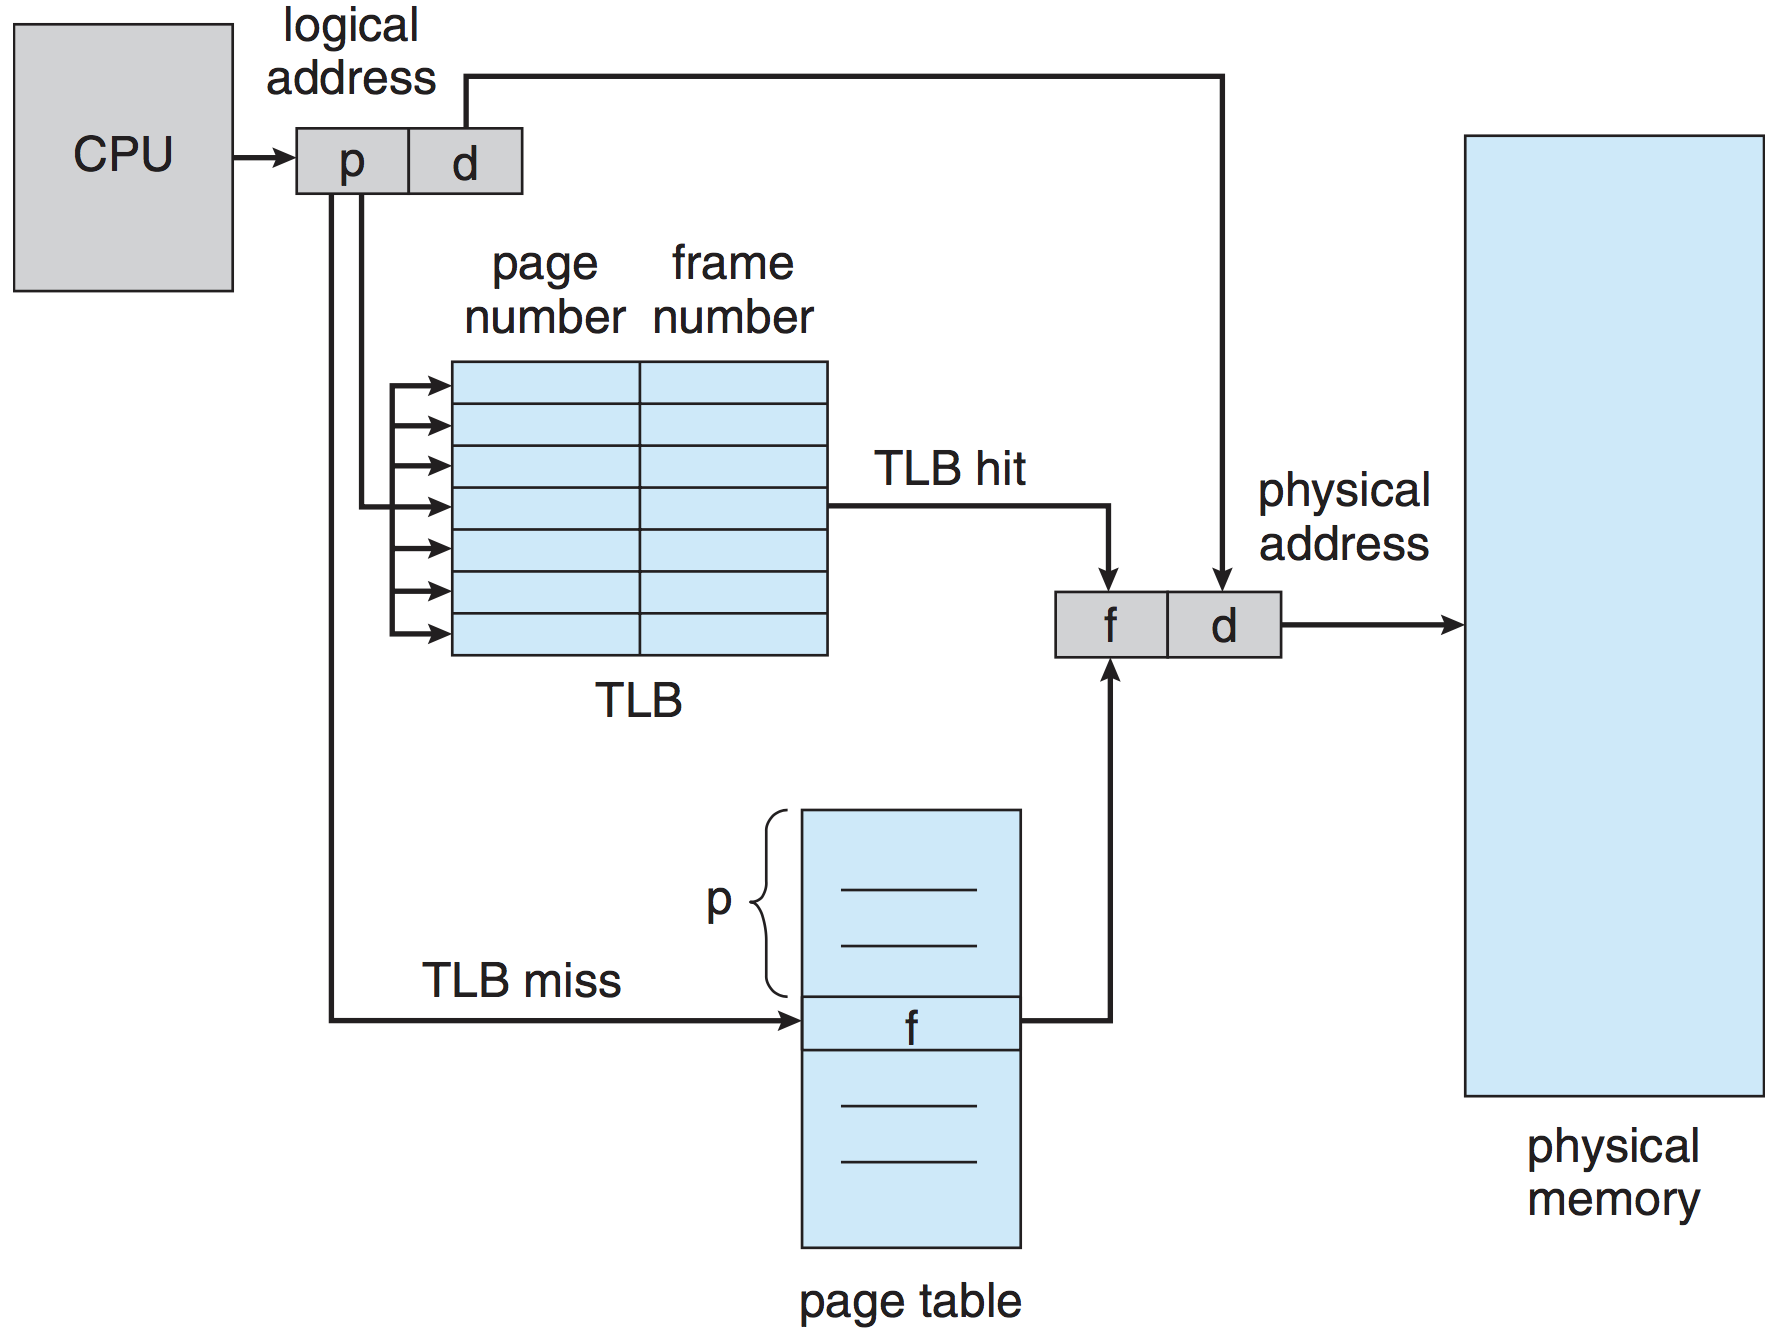
\includegraphics[width=0.7\textwidth]{page-table-2-tlb}
		\caption{Diagram of a TLB}
		\label{fig:paging:page-table-2-tlb}
	\end{figure}

& \textbf{Effective Access Time:} Amortized time for TLB lookup and page table access
	&& TLB hit ratio is proportional to the effective access time between the time for 1 memory access and the time for 2 memory accesses
	&& Equation:
	\end{easylist}
	\begin{align*}
		\textrm{ Let } t_m &= \textrm{ memory access time} \\
		\textrm{ Let } \varepsilon &= \textrm{ TLB lookup time (significantly less than } t_m \textrm{)} \\
		\textrm{ Let } \alpha &= \textrm{ TLB hit ratio (percentage of times page found in TLB)} \\
		\textrm{Effective Access Time }
		&= \textrm{ Time for TLB hit } \times \textrm{ TLB hit percentage } + \\
		& \textrm{ Time for TLB miss } \times \textrm{ TLB miss percentage } \\
		&= (\varepsilon + t_m) \times \alpha + (\varepsilon + 2 \times t_m) \times (1 - \alpha) \\
		&= \varepsilon + t_m \times (2 - \alpha) \\
	\end{align*}
	\begin{easylist}
	
		&&& Example:
		\end{easylist}
		\begin{align*}
			\textrm{ Let } t_m &= 100 \textrm{ ns} \\
			\textrm{ Let } \varepsilon &= 0 \\
			\textrm{ Let } \alpha &= 0.8 \\
			\textrm{Effective Access Time }
			&= \varepsilon + t_m \times (2 - \alpha) \\
			&= 100 \textrm{ ns } \times (2 - 0.8) \\
			&= 120 \textrm{ ns} \\
			\textrm{Slowdown } &= \frac{100 \textrm{ ns}}{120 \textrm{ ns}} - 1 = 20\% \\
		\end{align*}
		\begin{easylist}
	
		&&& Example:
		\end{easylist}
		\begin{align*}
			\textrm{ Let } t_m &= 100 \textrm{ ns} \\
			\textrm{ Let } \varepsilon &= 0 \\
			\textrm{ Let } \alpha &= 0.99 \\
			\textrm{Effective Access Time }
			&= \varepsilon + t_m \times (2 - \alpha) \\
			&= 100 \textrm{ ns } \times (2 - 0.99) \\
			&= 101 \textrm{ ns} \\
			\textrm{Slowdown } &= \frac{100 \textrm{ ns}}{101 \textrm{ ns}} - 1 = 1\% \\
		\end{align*}
		\begin{easylist}

& \textbf{Reentrant code:} Read-only code shared among multiple processes
	&& Must appear in the same location in the logical address spaces due to processes sharing a TLB

& Page table structural alternatives:
	&& Page table requires contiguous memory or the page table will need to be paged itself
	&& For an address space of $32$ bits and a page size of $4$ KB ($2^{12}$ bytes), a process could have $2^{32-12} = 2^{20}$ pages; for a page table with entries of $4$ bytes, the size of a page table for each process could be $2^{20} \times 4 = 2^{22} $ bytes $ = 4$ MB which is very large

	&& \textbf{Hierarchical page table:} Method to make page tables less contiguous in memory by paging a page table through partitioning the page table
		&&& Requires additional memory accesses
		&&& Diagram: See figure~\ref{fig:paging:page-table-3-hierarch}
		&&& Diagram of access: See figure~\ref{fig:paging:page-table-4-hierarch-access}

		\begin{figure}[!htb]
			\centering
			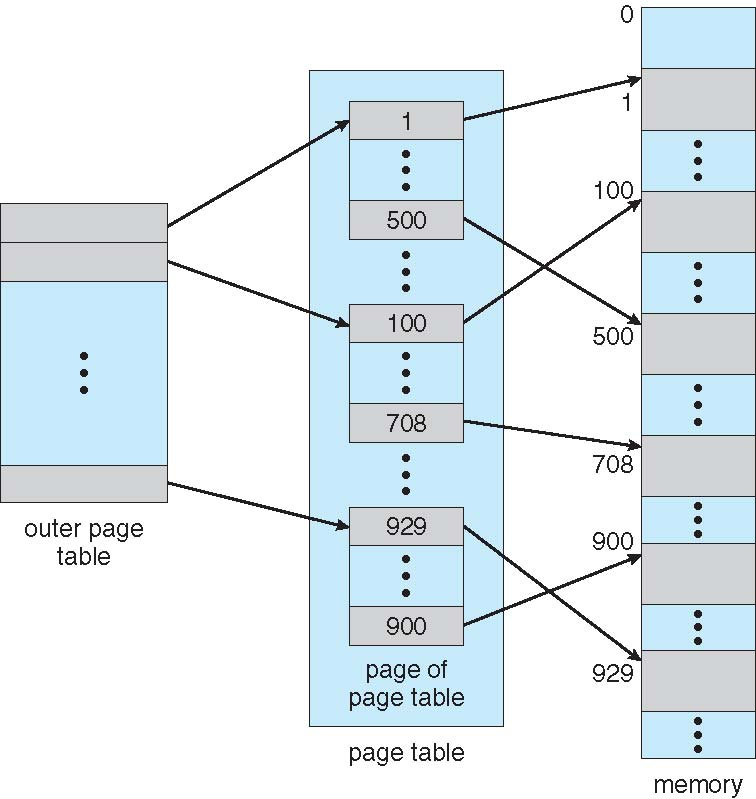
\includegraphics[width=0.7\textwidth]{page-table-3-hierarch}
			\caption{Diagram of a Hierarchical Page Table}
			\label{fig:paging:page-table-3-hierarch}
		\end{figure}
		&&& Diagram: See figure~\ref{fig:paging:page-table-3-hierarch}

		\begin{figure}[!htb]
			\centering
			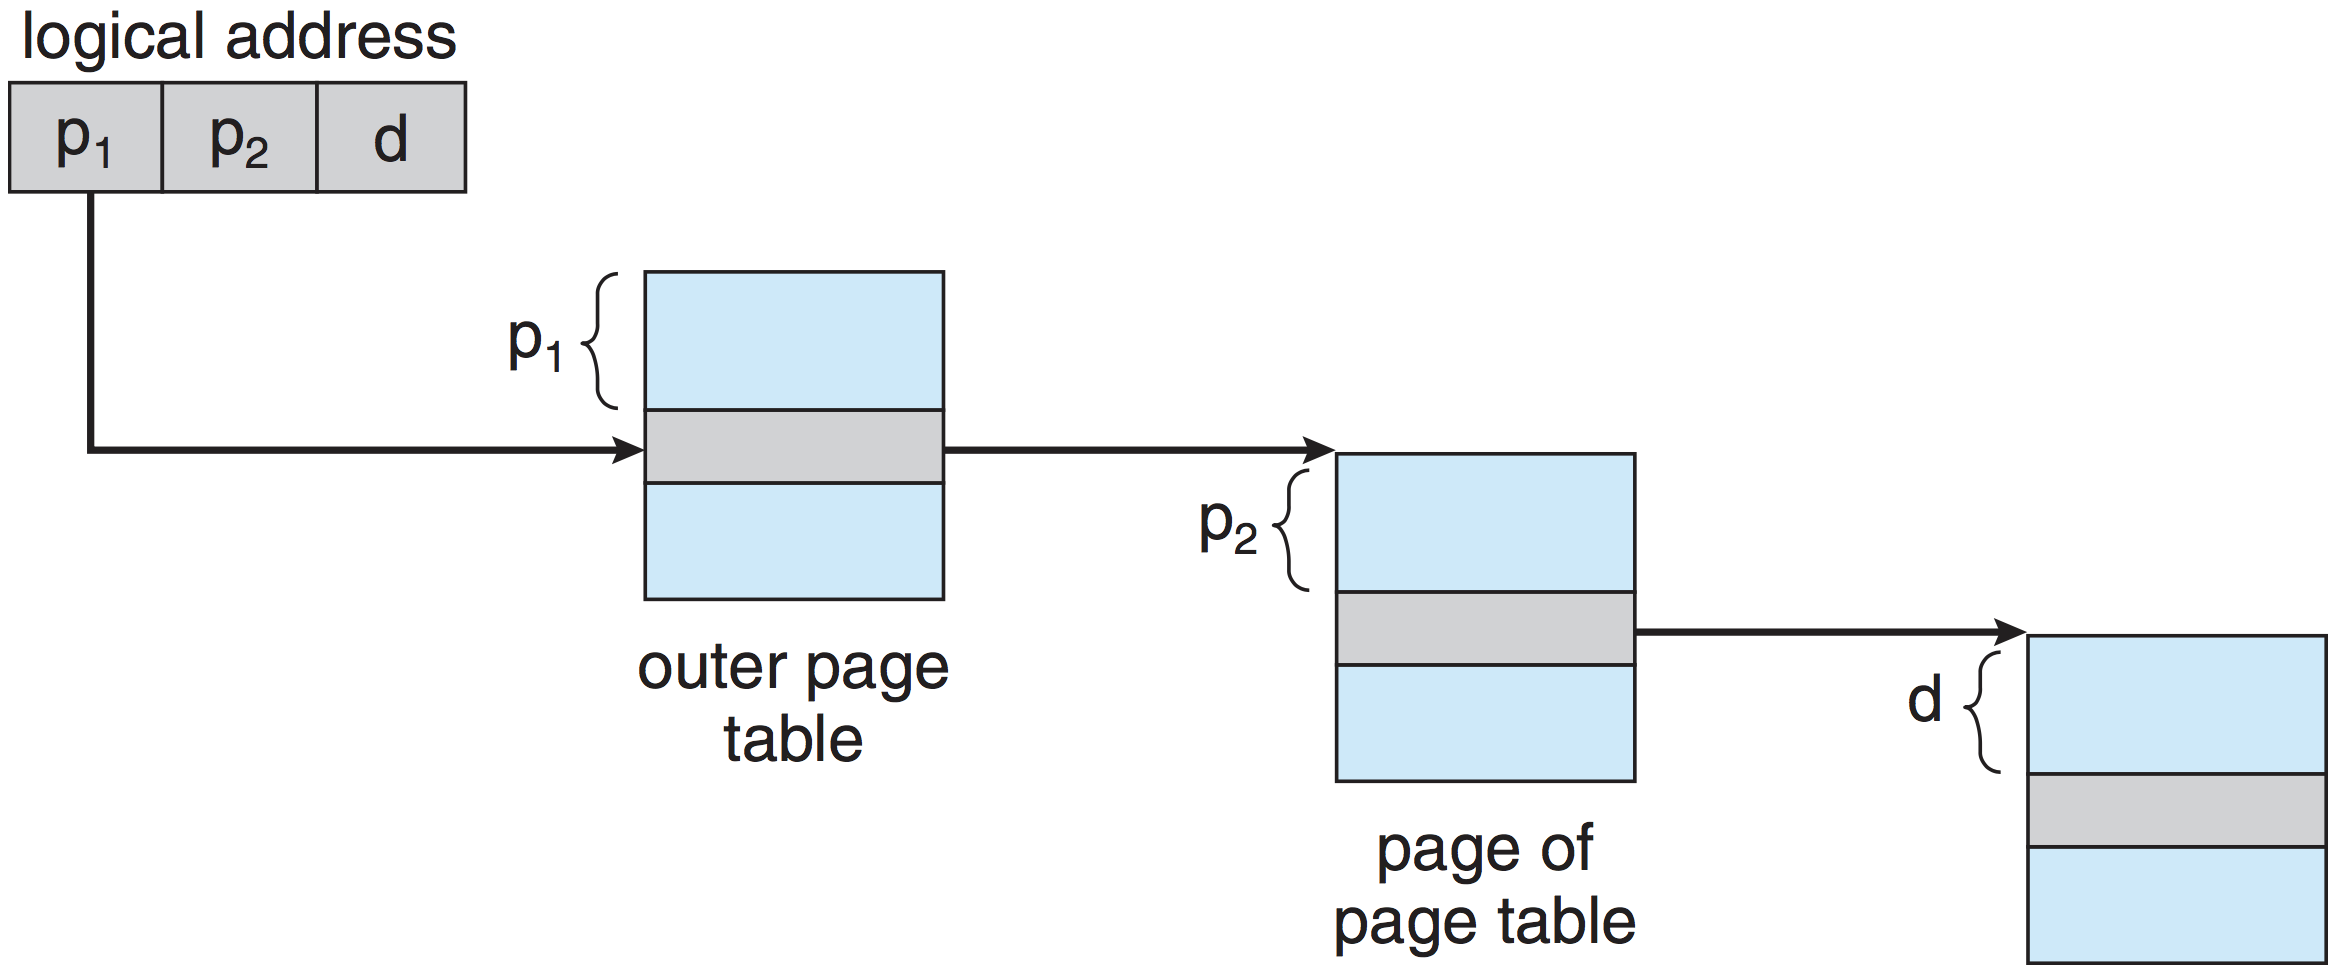
\includegraphics[width=0.7\textwidth]{page-table-4-hierarch-access}
			\caption{Accessing a Hierarchical Page Table}
			\label{fig:paging:page-table-4-hierarch-access}
		\end{figure}

	&& \textbf{Hashed page table:} Method to store page table entries non-contiguously by hashing page number to a linked list of elements, each with a page number and associated frame number
		&&& Diagram: See figure~\ref{fig:paging:page-table-6-inverted}

		\begin{figure}[!htb]
			\centering
			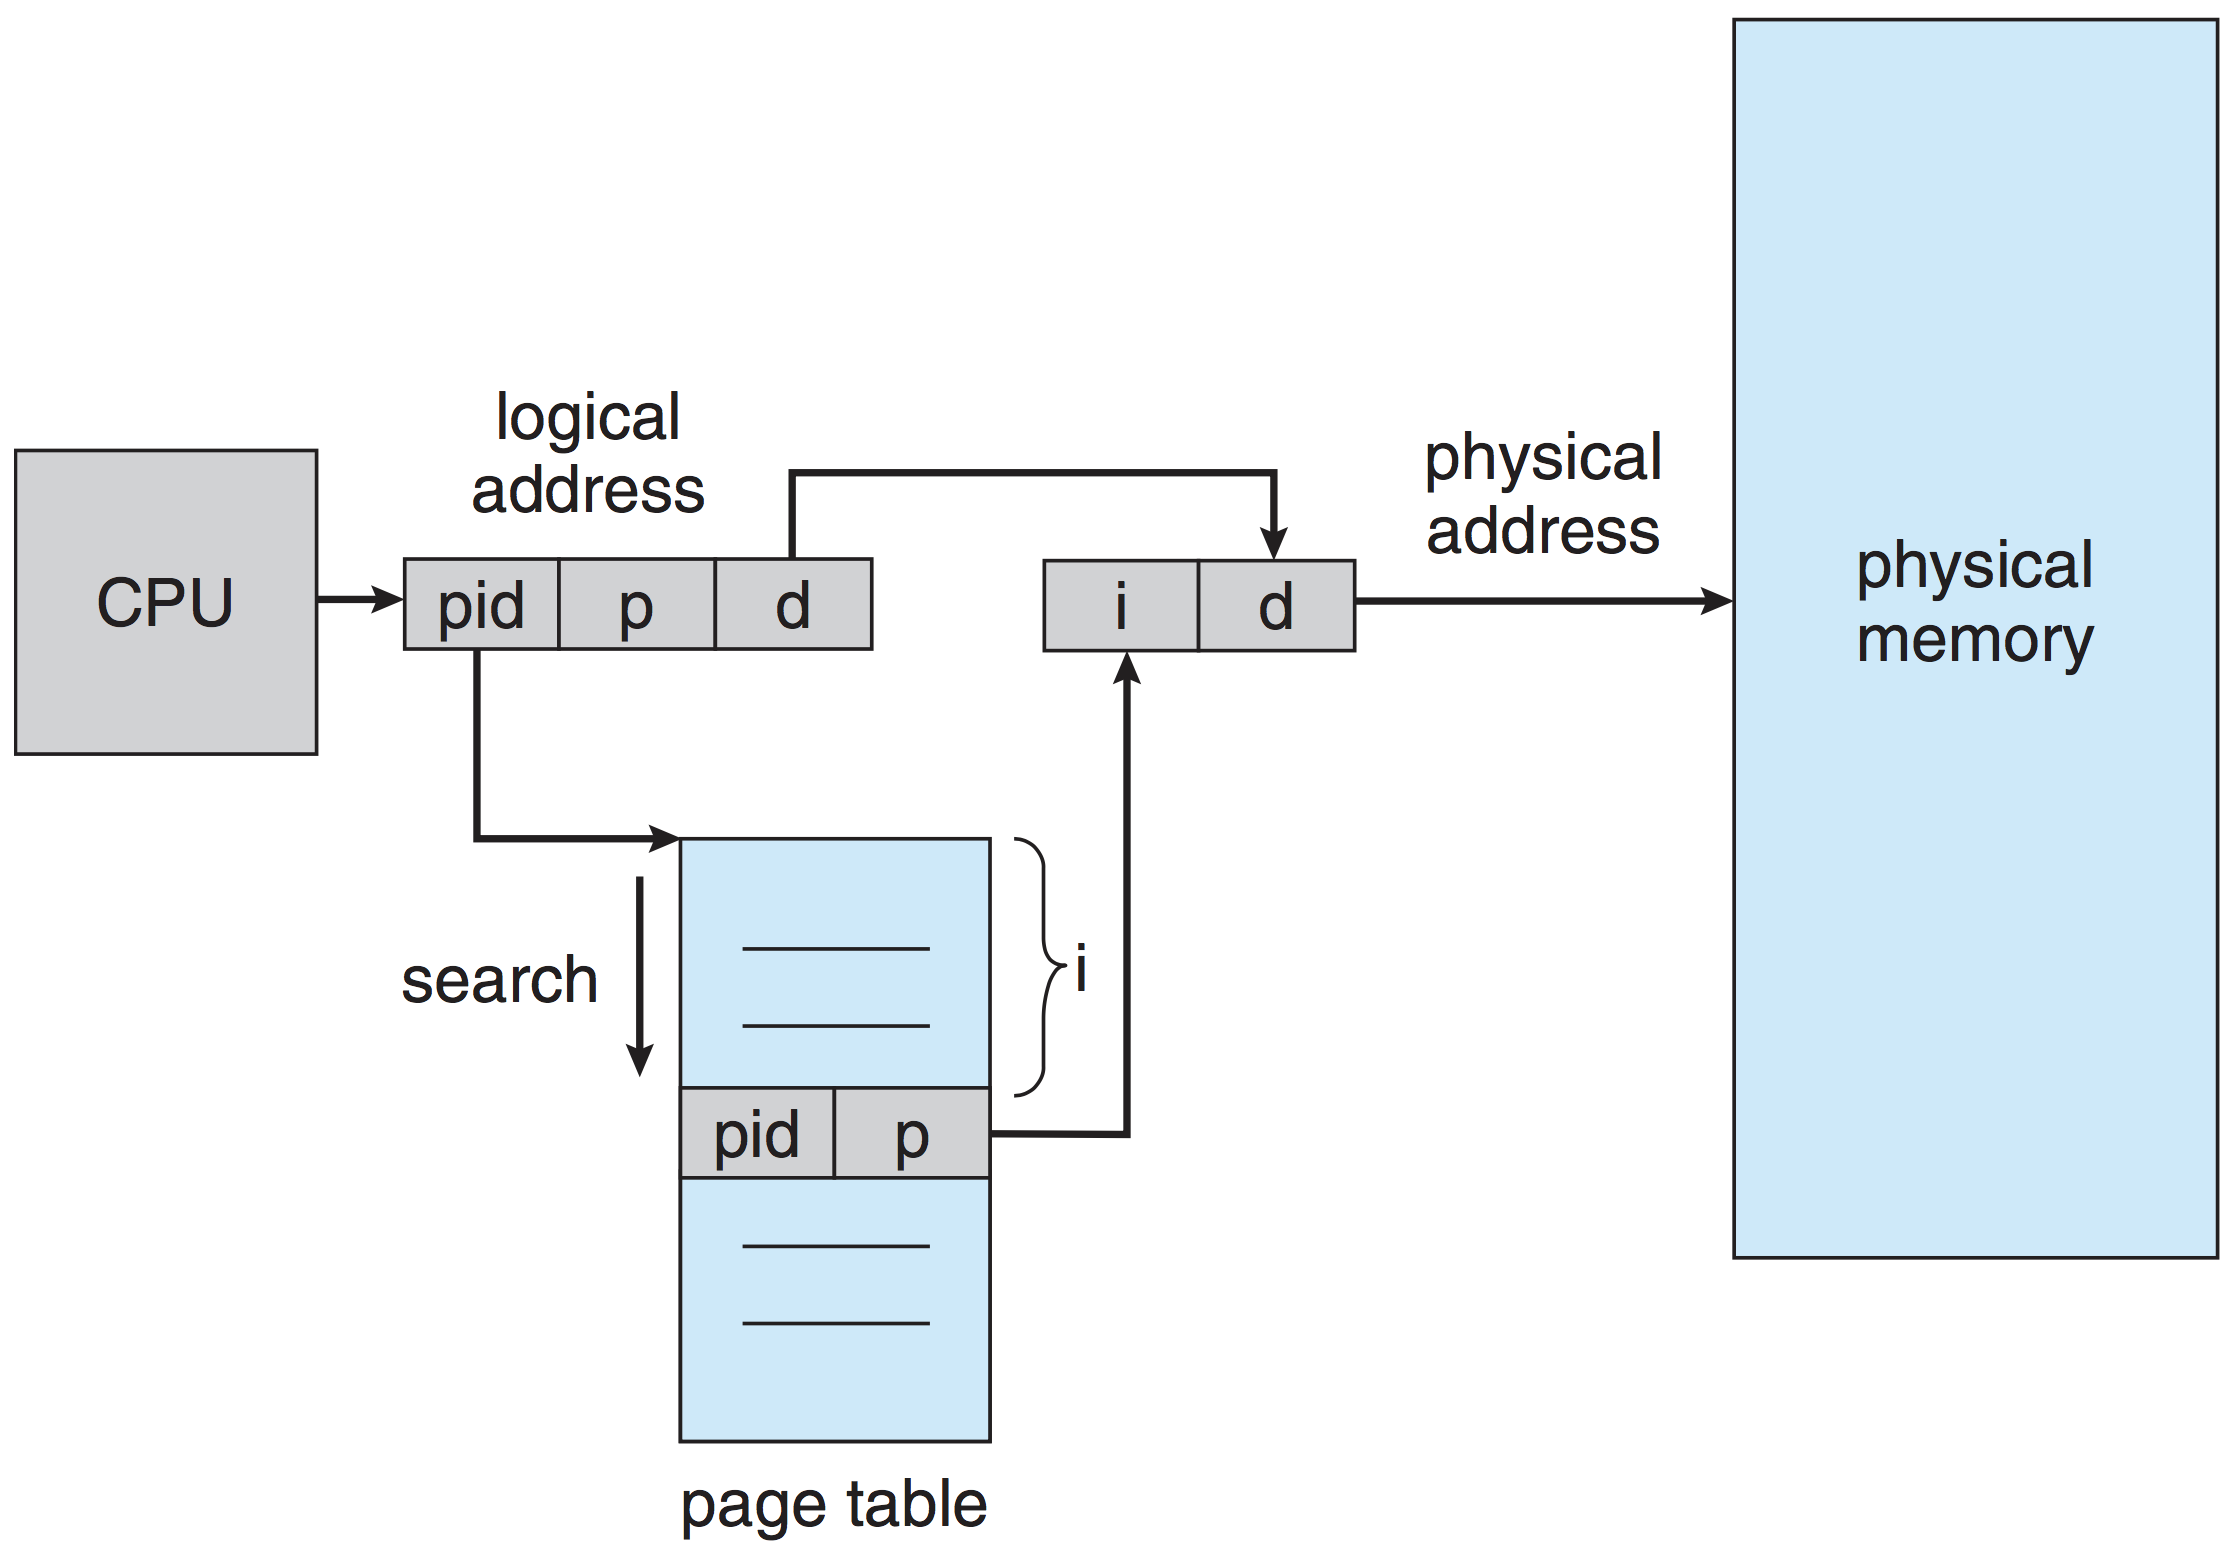
\includegraphics[width=0.7\textwidth]{page-table-6-inverted}
			\caption{Diagram of an Inverted Page Table}
			\label{fig:paging:page-table-6-inverted}
		\end{figure}
		
	&& \textbf{Inverted page table:} Method to use only one page table for all processes by using a table of page numbers (limited by amount of frames) and the process which owns the frame
		&&& Increases time to find a page reference
		&&& Creates difficulty in implementing a shared page

& \textbf{Internal fragmentation:} Situation where memory allocated as a fixed-size partition is larger than required which creates unusable excess memory

\end{easylist}
\subsection{Segmentation}
	\label{subsec:memory-management:segmentation}
\begin{easylist}

& \textbf{Segment:} Component of a program (e.g. function, object, main program)
	&& Segments are paged to avoid external fragmentation so the user interacts with the segments and the OS interacts with the pages

& \textbf{Segment table:} Structure which maps a logical address to a physical address using a base address and limit

\end{easylist}
\clearpage
	%
% CMPT 300: Operating Systems I - A Course Overview
% Section: Virtual Memory
%
% Author: Jeffrey Leung
%

\section{Virtual Memory}
	\label{sec:virtual-memory}
\begin{easylist}

& \textbf{Virtual memory:} Abstraction of memory management where logical memory can be conceptually larger than the physical address space
	&& Only part of a program is in memory at any given time

& \textbf{Demand paging:} Making pages available in virtual memory only as needed
	&& Decreases I/O requirements and waiting time, and increases number of potential concurrent processes
	&& Indicated by valid-invalid bit in page table (if invalid, the memory access is either illegal or not yet in memory)

\end{easylist}
\subsection{Page Faults}
	\label{subsec:virtual-memory:page-faults}
\begin{easylist}

& \textbf{Page fault:} Legal memory access of a page which is not currently in memory which triggers retrieval
	&& \textbf{Major page fault:} Page is brought from disk
	&& \textbf{Minor page fault:} Page table is updated (e.g. linking shared pages)
	&& If no free pages are available, a page will be removed from memory to make room
	&& To preserve atomicity of instructions which modify data, previous register values are saved and hardware accesses both ends of the data before execution to trigger page faults
	&& Effective Access Time:
	\end{easylist}
	\begin{align*}
		\textrm{Let } p &= \textrm{ page fault rate, } 0 \leq p \leq 1 \\
		& \textrm{ where 0 is no faults, 1 is every reference is a fault} \\
		\textrm{Let } t_m &= \textrm{ memory access time} \\
		\textrm{Let } t_p &= \textrm{ page fault time} \\
		& \textrm{(including interrupt, page read, restart)} \\
		\textrm{Effective access time }
		&= p \times t_p + (1 - p) \times t_m \\
	\end{align*}
	\begin{easylist}

		&&& Example:
		\end{easylist}
		\begin{align*}
			p &= 0.001 \textrm{ 1 fault per 1,000 memory accesses} \\
			t_m &= 200 \textrm{ ns} \\
			t_p &= 8 \textrm{ ms} = 8,000,000 \textrm{ ns}\\
			\textrm{Effective access time }
			&= p \times t_p + (1 - p) \times t_m \\
			&= 0.001 \times 8,000,000 + (1 - 0.001) \times 200 \\
			&= 8,000 + 199.8 \\
			&= 8,200 \textrm{ ns} \\
			\textrm{Slowdown } &= \frac{8200 \textrm{ ns}}{200 \textrm{ ns}} = 40 \textrm{ times slower}
		\end{align*}
		\begin{easylist}
		
	&& Process:
		&&& Send a trap to the OS
		&&& Save the user registers and process states
		&&& Determine that the interrupt was a page fault
		&&& Check legality of the page access and determine the location of the page
		&&& Issue a read from the disk to a free frame
		&&& Wait until the read request is serviced, with seek and/or latency time
		&&& Transfer the page to a free frame
		&&& While waiting, allocate the CPU to some other process
		&&& Receive a completion interrupt from the disk I/O subsystem
		&&& Save the registers and process state for the other process
		&&& Determine that the interrupt was from the disk
		&&& Correct the page tables to show page is now in memory
		&&& Wait for the CPU to be allocated to this process again
		&&& Restore the user registers, process state, and new page table
		&&& Resume the interrupted instruction

& \textbf{Copy-on-Write (COW):} Method of quickly/efficiently creating a child process by sharing the pages of the parent process in memory and copying the data only when a shared page is modified

& \textbf{Pre-paging:} Bringing pages into memory before they are referenced to decrease page faults
	&& May waste memory and I/O if the page is not used

\end{easylist}
\subsection{Page Replacement}
	\label{subsec:virtual-memory:page-replacement}
\begin{easylist}

& \textbf{Page replacement algorithm:} Method of selecting a victim page to be removed from memory which is designed to minimize fault rate
	&& Dirty/modified bit in page table entries to save swap-out overhead if the victim page was not modified
	&& \textbf{I/O interlock:} Page currently used for I/O is locked in memory and cannot be replaced during a fault

& \textbf{First-In-First-Out (FIFO) page replacement algorithm:} Removing from memory the oldest page upon a fault
	&& Could consistently remove a heavily-used page
	&& \textbf{Bélády's anomaly:} Phenomenon in the FIFO page replacement algorithm where increasing available frames may potentially result in greater page faults
	
& \textbf{Least Recently Used (LRU) page replacement algorithm:} Removing from memory the page which has not been used for the longest period, upon a page fault
	&& Counter tracking: Using a data field to store CPU clock of the last memory access and searching for the oldest page
		&&& Search is time-consuming, many memory writes, potential clock overflow, requires hardware
	&& Stack tracking: Using a stack created from a doubly-linked list for which each page access moves the page to the top
		&&& Memory reference updating is expensive, requires hardware
		&&& No search is required

& \textbf{Second-chance/clock replacement:} Using a set of reference bits which are set when a page is referenced and reset when a page is replaced, and removing a page which was not used since the last replacement

& \textbf{Least Frequently Used (LRU) page replacement algorithm:} Removing from memory the page which has been used the least
	&& Removes pages which are not used often
	&& Early heavily-used pages will stay in memory
& \textbf{Most Frequently Used (MRU) page replacement algorithm:} Removing from memory the page which has been used the most
	&& Pages with smaller counts are estimated to be newer and kept
	&& Heavily-used pages may be removed more frequently

& \textbf{Optimal page replacement algorithm:} Removing from memory the page which will not be used for the longest period of time, upon a fault
	&& Only possible in theory or when analyzing a past set of page accesses
	&& Used to benchmark existing algorithms

\end{easylist}
\subsection{Frame Allocation}
	\label{subsec:virtual-memory:frame-allocation}
\begin{easylist}

& \textbf{Equal allocation:}

& \textbf{Proportional allocation:} Allocating frames per process relative to the size of the process
	&& Formula:
	\end{easylist}
	\begin{align*}
		\textrm{Let } m &= \textrm{ total number of frames} \\
		\textrm{Let } p_i & \textrm{ be a given process} \\
		\textrm{Let } s_i &= \textrm{ size of process } p_i \\
		\textrm{Page allocation } a_i \textrm{ for } p_i
		&= \frac{s_i}{\sum s_i} \times m
	\end{align*}
	\begin{easylist}
	
		&&& Example:
		\end{easylist}
		\begin{align*}
			m &= 64 \textrm{ frames} \\
			s_1 \textrm{ for process } p_1 &= 10 \\
			s_2 \textrm{ for process } p_2 &= 127 \\
			\textrm{Page allocation } a_1
			&= \frac{s_1}{\sum s_1} \times m \\
			&= \frac{10}{10+127} \times 64 \\
			&\approx 5
		\end{align*}
		\begin{easylist}

& \textbf{Priority allocation:} Allocating frames per process relative to the priority of the process

& \textbf{Global replacement:}
& \textbf{Local replacement:}

& \textbf{Locality model:} Keeping in memory the pages necessary for the current segment of code

& \textbf{Working set:}
	&& Managed with an interval timer and set of reference bits (per page in memory), which is set when a page is referenced

& \textbf{Thrashing:} Situation where a process is starved of necessary frame allocations and must constantly swap pages

\end{easylist}
\subsection{Kernel Memory Allocation}
	\label{subsec:virtual-memory:kernel-memory-allocation}
\begin{easylist}

& \textbf{Buddy system:} Allocating memory from fixed-size contiguous segments with size to the power of 2
	&& May have up to 50\% internal fragmentation
& \textbf{Slab allocator:} Allocating memory from precreated spaces for kernel data structures
	&& \textbf{Cache:} Paged instantiation space in memory for an object
	&& \textbf{Slab:} Contiguous memory which contains multiple caches
	&& Memory allocation is fast and has no fragmentation

& \textbf{Memory mapping:} Mapping a file to a memory address space so modifications have the behaviour of ordinary memory accesses

\end{easylist}
\clearpage

	%
% CMPT 300: Operating Systems I - A Course Overview
% Section: Filesystems
%
% Author: Jeffrey Leung
%

\section{Filesystems}
	\label{sec:filesystems}
\begin{easylist}

& Cyclic links can cause infinite loops during searches

& Mounting:
	&& 

\end{easylist}
\clearpage

\end{document}